% a-project.tex, v-1.0.3 marcoreis baseado no
% abntex2-modelo-trabalho-academico.tex, v-1.9.7 laurocesar
% Copyright 2012-2018 by abnTeX2 group at http://www.abntex.net.br/ 
% 
% This work consists of the files ........
% 
% -----------------------------------------------------------------------------
% Modelo para desenvolvimento de documentação de projetos acadêmicos
% (tese de doutorado, dissertação de mestrado e trabalhos de monografias em geral) 
% em conformidade com ABNT NBR 14724:2011: Informação e documentação. 
% -----------------------------------------------------------------------------
% Opções para a documentação
%
% Fancy page headings 
%\documentclass[fancyheadings, subook]{Classes/a-prj}
%\documentclass[fancyheadings, sureport]{Classes/a-prj}
%
% Fancy chapters and sections headings 
%\documentclass[fancychapter, subook]{Classes/a-prj}
%\documentclass[fancychapter, sureport]{Classes/a-prj}
%
% Fancy page , chapters and sections headings
%\documentclass[fancyheadings, fancychapter, subook]{Classes/a-prj}
\documentclass[fancyheadings, fancychapter, sureport]{Classes/a-prj}
%
% -----------------------------------------------------------------------------
% Alguns comandos para a fancy page headings)
%
% Page header line width
%\footlinewidth{value}
%
% Page footer line width
%\headlinewidth{value}
%
% Page header and footer line width
%\headingslinewidth{value}
%
% Page header and footer lines without text
%\headingslinesonly
%
% The default line width is 0.3pt.
% Set the value to 0pt to remove the page header and/or footer line
%
% -------------------------------------------------------------------------------
% Formato de figuras suportado
% -------------------------------------------------------------------------------
% O formato das figuras depende da forma como o arquivo de saída é gerado.
% As figuras inseridas na pasta Figures serão automaticamente reconhecidas sem
% a necessidade de inserir a extensão do arquivo.
%
% O pdfLaTEX (PDF) suporta figuras com as extensões: pdf, jpg, png e mps.
%
% -------------------------------------------------------------------------------
% Árvore do diretório a-project.tex
%  Diretório
%       \Classes        (requerido)
%       \Figures        (requerido) --------------------------------->
%       \Figures\PDF    (optional)
%       \Figures\JPG    (optional) Figures located within these
%       \Figures\PNG    (optional) folders are searched automatically
%       \Figures\MPS    (optional)  by the a-prj class.
%       \Figures\EPS    (optional)
%       \Figures\PS     (optional) <--------------------------------
%       \Tables         (requerido)
%       \Others         (requerido)
%       \Chapters       (requerido)
%       \Appendices     (optional)
%       \References     (requerido)
%
% -------------------------------------------------------------------------------
% PDF File resumo
\ifpdf
    \hypersetup{
    	backref,
        colorlinks  = true,
        pdftitle    = Modelo de documentação,
        pdfauthor   = {Marco Reis, marco.a.reis@gmail.com},
        pdfsubject  = Mestre em Engenharia,
        pdfcreator  = Subtitulo,
        pdfproducer = PDFLatex,
        pdfkeywords = {documentação, latex, dissertação, tese}}
 \fi
%
% -------------------------------------------------------------------------------
% Relação de pacotes opcionais utilizados
\usepackage[utf8]{inputenc}
\usepackage[brazil]{babel}
\usepackage{longtable}
\usepackage{dcolumn}
\usepackage{multirow}
\usepackage{lscape}
%\usepackage{graphicx}
\usepackage{rotating}
%\usepackage{float,subfigure}
%\usepackage{graphicx, subfigure}
\usepackage{cite}
\usepackage[left=3cm,top=3cm,right=2cm,bottom=2cm]{geometry}
\usepackage[alf]{abntex2cite}
\usepackage{ifpdf}
\usepackage{shadow}
\usepackage{wrapfig}
\usepackage[normalem]{ulem}
\usepackage{makeidx}
\usepackage{yfonts}
\usepackage{algorithm}
\usepackage{algorithmic}
\usepackage{lmodern}
\usepackage[T1]{fontenc}
\usepackage{indentfirst}
\usepackage{color}
\usepackage{microtype}
\usepackage{lipsum}
\usepackage{caption}
\usepackage{subcaption}
%
\makeindex 
\setlength{\LTcapwidth}{\textwidth}
%
\newtheorem{theorem}{Teorema}
\newtheorem{definition}[theorem]{Definição}
%
% -------------------------------------------------------------------------------
% Configurações do pacote backref
\renewcommand{\backrefpagesname}{Citado na(s) página(s):~}
% Texto padrão antes do número das páginas
\renewcommand{\backref}{}
% Define os textos da citação
\renewcommand*{\backrefalt}[4]{
	\ifcase #1 %
		Nenhuma citação no texto.%
	\or
		Citado na página #2.%
	\else
		Citado #1 vezes nas páginas #2.%
	\fi
}
% 
% -------------------------------------------------------------------------------
% Início do documento raiz
\begin{document}
% Definição do título da página
    \university{Centro Universitário SENAI CIMATEC}
	%\faculty{Programa de...}
	%\school{Escola de...}
% 
    %\course{Engenharia Elétrica}
    \typework{Relatório do Projeto Walker}
% 
	%\course{Mestrado em Modelagem Computacional e Tecnologia Industrial}
	%\typework{Disserta\c{c}\~ao de mestrado}
	%\typework{Exame de Qualificação de Mestrado}
% 
	%\course{Engenharia Elétrica}
	%\typework{Tese de doutorado}
	%\typework{Exame de Qualificação de doutorado}
%
% -------------------------------------------------------------------------------
% Informações gerais
    \thesistitle{Walker: um robô bípede}
    \hidevolume
    \thesisvolume{Volume 1 of 1}
    \thesisauthor{Brenda Alencar}
    \thesisauthorr{Felipe Mohr}

    \thesisadvisor{Prof. Marco Reis, M.Eng.}
    %\hidecoadvisor
    %\thesiscoadvisor{Marco Reis}
    \thesisdegreetitle{Bacharel em Engenharia}
    \thesismonthyear{Agosto de 2020}
% 
    \maketitlepage
%
% ----------------------------------------------------------------------------
% Inserir Folha de rosto, Nota de estilo, folha de assinaturas, dedicatoria
    \begin{folharosto}

\begin{center}
\theauthor \\
\theauthorr \\
%\theauthorrr \\
%\theauthorrrr \\
%\theauthorrrrr \\
\end{center}
\ \\
\ \\
\ \\
\ \\
\ \\
\begin{spacing}{2}
   \begin{center}
   {\LARGE {\bf \thetitle}}
   \end{center}
\end{spacing}
\ \\
\ \\
\ \\
\vspace*{85mm}
% \begin{flushright}

%    \begin{list}{}{
%       \setlength{\leftmargin}{7.5cm}
%       \setlength{\rightmargin}{0cm}
%       \setlength{\labelwidth}{0pt}
%       \setlength{\labelsep}{\leftmargin}}

%       \item \thetypework apresentada ao \thefaculty, Curso de \thecourse
%       do \theuniversity, como requisito parcial para a obten\c{c}\~ao do
%       t\'itulo de {\bf \thedegreetitle}.

%       \begin{list}{}{
%       \setlength{\leftmargin}{0cm}
%       \setlength{\rightmargin}{0cm}
%       \setlength{\labelwidth}{0pt}
%       \setlength{\labelsep}{\leftmargin}}

%       \item \'Area de conhecimento: Interdisciplinar

%       \item Orientador: \theadvisor
%       \newline \hspace*{2.1cm}  %{\it \theuniversity}

%       \end{list}
%    \end{list}

% \end{flushright}
\ \\
\ \\
\ \\
\ \\
%\begin{spacing}{1.5}
   \begin{center}
   Salvador \par
   \theuniversity \par
   2020
   \end{center}
%\end{spacing}

\end{folharosto}

    %\include{Others/NotaEstilo}
    %\include{Others/FolhaAssinaturas}
    %\include{Others/dedicatoria}
    %\include{Others/agradecimentos}
%
% ----------------------------------------------------------------------------
% Resumo/abstract, sumário e siglas
    \begin{romanpagenumbers}
        \include{Others/resumo}
        \include{Others/abstract}
        % Make list of contents, tables and figures
        \thesiscontents
        %Include other required section
        %\include{Others/abbreviation}
        %\include{Others/simbolos}
        %Switch the page numbering back to the default format
    \end{romanpagenumbers}
%
% ---------------------------------------------------------------------------
% Include thesis chapters
    \parskip=\baselineskip
    \chapter{Introdução}
\label{chap:intro}

Este pode ser um parágrafo citado por alguém \cite{Barabasi2003-1}.

%--------- NEW SECTION ----------------------
\section{Objetivos}
\label{sec:obj}
Este projeto consiste em desenvolver um robô bípede de pequeno porte, ou seja que se desloca sobre dois pés. O robô deve ser capaz de se locomover e desviar de obstáculos em um determinado ambiente. 


\subsection{Objetivos Específicos}
\label{ssec:objesp}
Os objetivos específicos deste projeto são:
\begin{itemize}
      \item Desenvolver habilidades de gestão de projetos.
      \item Desenvolver algoritmos utilizando ROS;
      \item Utilizar visão computacional;
      \item Simular um robô no gazebo;
  \end{itemize}



%--------- NEW SECTION ----------------------
\section{Justificativa}
\label{sec:justi}

O pesquisador/estudante deve apresentar os aspectos mais
relevantes da pesquisa ressaltando os impactos (e.g. cient\'ifico,
tecnol\'ogico, econ\^omico, social e ambiental) que a pesquisa
causar\'a. Deve-se ter cuidado com a ingenuidade no momento em que
os argumentos forem apresentados.




%--------- NEW SECTION ----------------------
\section{Organização do documento}
\label{section:organizacao}

Este documento apresenta $5$ capítulos e está estruturado da seguinte forma:

\begin{itemize}

  \item \textbf{Capítulo \ref{chap:intro} - Introdução}: Contextualiza o âmbito, no qual a pesquisa proposta está inserida. Apresenta, portanto, a definição do problema, objetivos e justificativas da pesquisa e como este \thetypeworkthree está estruturado;
  \item \textbf{Capítulo \ref{chap:fundteor} - Fundamentação Teórica}: XXX;
  \item \textbf{Capítulo \ref{chap:metod} - Materiais e Métodos}: XXX;
  \item \textbf{Capítulo \ref{chap:result} - Resultados}: XXX;
  \item \textbf{Capítulo \ref{chap:conc} - Conclusão}: Apresenta as conclusóes, contribuições e algumas sugestões de atividades de pesquisa a serem desenvolvidas no futuro.

\end{itemize}

    \chapter{Desenvolvimento do projeto}
\label{chap:fundteor}
%--------- NEW SECTION ----------------------
 Nesta seção será descrito o procedimento utilizado para construção inicial do robô Walker, incluindo as fases conceitual e design.  Será apresentado a ideação do projeto, especificações e as funcionalidades.

\section{Descrição}
 O Walker é um robô bípede, ou seja, um robô que se desloca sobre dois pés. Este deve 

\subsection{Requisitos do cliente}
\subsection{Arquitetura Geral}
\subsection{Requisitos técnicos}
\label{sec:sota}
\lipsum[1]

%---------------picture------------------------------------
\begin{figure} [h!]												 
	\centering													 
	\includegraphics[width=0.6\textwidth]{./lq}				 
	\caption{Insufficient data.}		
	\label{img:ihuma}												 
\end{figure}													 
%----------------------------------------------------------

%--------- NEW SECTION ----------------------
\section{Assunto 1}
\label{sec:ass1}
\lipsum[1]



%---------------picture------------------------------------
% \begin{figure}
%     \centering
%     \subfigure[Figure A]{\label{fig:a}\includegraphics[width=60mm]{./lq}}
%     \subfigure[Figure B]{\label{fig:b}\includegraphics[width=60mm]{./lq}}
%     \subfigure[Figure C]{\label{fig:c}\includegraphics[width=\textwidth]{./lq}}
%     \caption{Three simple graphs}
%     \label{fig:three graphs}
% \end{figure}
%----------------------------------------------------------

\begin{figure}
    \centering
    \begin{subfigure}[b]{0.3\textwidth}
        \centering
        \includegraphics[width=\textwidth]{./lq}
        \caption{$y=x$}
        \label{fig:y equals x}
    \end{subfigure}
    \hfill
    \begin{subfigure}[b]{0.3\textwidth}
        \centering
        \includegraphics[width=\textwidth]{./lq}
        \caption{$y=3sinx$}
        \label{fig:three sin x}
    \end{subfigure}
    \hfill
    \begin{subfigure}[b]{0.3\textwidth}
        \centering
        \includegraphics[width=\textwidth]{./lq}
        \caption{$y=5/x$}
        \label{fig:five over x}
    \end{subfigure}
       \caption{Three simple graphs}
       \label{fig:three graphs}
\end{figure}


%--------- NEW SECTION ----------------------
\section{Assunto 2}
\label{sec:ass2}
flkjasdlkfjasdlkfjs

\begin{table}[h]
    \begin{subtable}[h]{0.45\textwidth}
        \centering
        \begin{tabular}{l | l | l}
        Day & Max Temp & Min Temp \\
        \hline \hline
        Mon & 20 & 13\\
        Tue & 22 & 14\\
        Wed & 23 & 12\\
        Thurs & 25 & 13\\
        Fri & 18 & 7\\
        Sat & 15 & 13\\
        Sun & 20 & 13
       \end{tabular}
       \caption{First Week}
       \label{tab:week1}
    \end{subtable}
    \hfill
    \begin{subtable}[h]{0.45\textwidth}
        \centering
        \begin{tabular}{l | l | l}
        Day & Max Temp & Min Temp \\
        \hline \hline
        Mon & 17 & 11\\
        Tue & 16 & 10\\
        Wed & 14 & 8\\
        Thurs & 12 & 5\\
        Fri & 15 & 7\\
        Sat & 16 & 12\\
        Sun & 15 & 9
        \end{tabular}
        \caption{Second Week}
        \label{tab:week2}
     \end{subtable}
     \caption{Max and min temps recorded in the first two weeks of July}
     \label{tab:temps}
\end{table}
    \chapter{Desenvolvimento do projeto}
Nesta seção será descrito o procedimento utilizado para construção inicial do robô Walker, incluindo as fases conceitual e design.  Será apresentado a ideação do projeto, especificações e as funcionalidades.

\section{Ideação}
%escrever oq sera apresentado

\subsection{Arquitetura Geral}
 A arquitetura geral, apresentada na Figura \ref{fig:Arquitetura geral}, relaciona de modo geral a interface do usuário, com a central de gerenciamento do sistema e com a interface com hardware. Neste contexto, a interface do usuário representa o contato direto com o usuário por meio de um botão \textit{on/off}, um \textit{joystick} e por acesso remoto, através de um computador devidamente conectado.

 \begin{figure} [h!]	
    \centering

    \caption{Arquitetura Geral}
    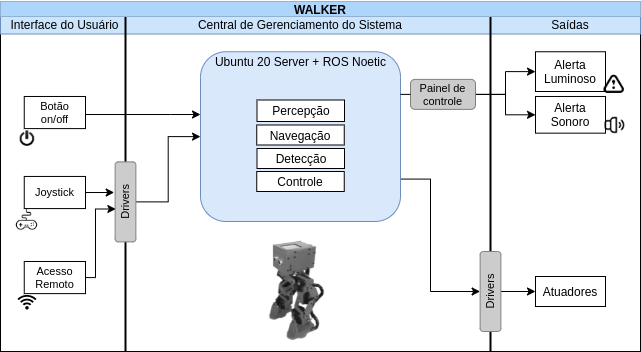
\includegraphics[width=0.8\textwidth]{general_architecture}
    \caption*{Fonte: Autoria própria.}
    \label{fig:Arquitetura geral}
\end{figure}	

Para a central de gerenciamento do sistema utilizou-se o sistema operacional \textit{Ubuntu} 20.04 junto ao framework de robótica ROS \textit{Noetic}. Neste cojunto se encontram as principais funcionalidades do robô: percepção, navegação, detecção e controle. Por fim, no conjunto de saídas estão os atuadores e os alertas sonoro e luminoso.

\subsection{Requisitos técnicos}

%desdobramento da função qualidade
\subsection{Quality Function Deployment}
\textit{Quality Function Deployment} é uma ferramenta de qualidade que auxilia na conversão das demandas do cliente em características de qualidade do produto. Dessa forma, no primeiro ciclo do QFD foram analisados os requisistos do cliente e os requisitos técnicos necessários, sinalizando os pontos mais importantes e as relações entre estes. O resultado foi exposto na \ref{fig:QFD}

\begin{figure} [h!]	
    \centering
    \caption{ Primeiro ciclo QFD}
    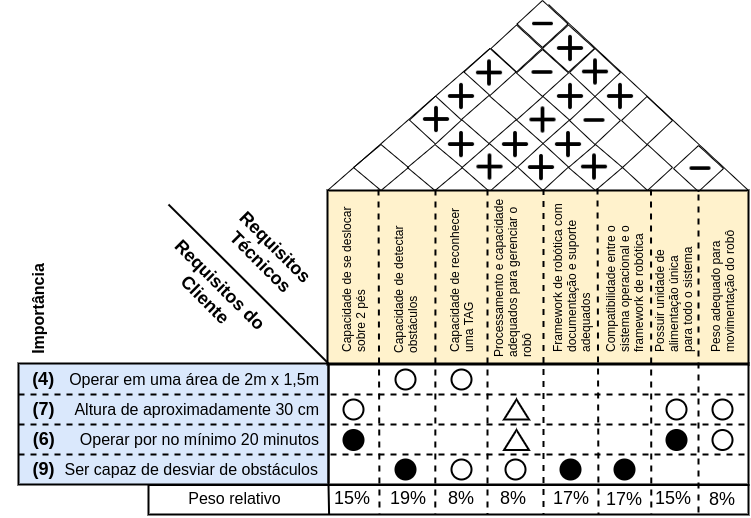
\includegraphics[width=0.8\textwidth]{Figures/QFD}
    \caption*{Fonte: Autoria própria.}
    \label{fig:QFD}
\end{figure}
 Através do QFD foi possível observar 

% %--------- NEW SECTION ----------------------
% \section{Interface do Usuário}
% \label{sec:ui}
% \lipsum[1]

% %--------- NEW SECTION ----------------------
% \section{Simulação do sistema}
% \label{sec:sim}
% \lipsum[2-4]


    \include{Chapters/resultados}
    \include{Chapters/conclusao}
    % include more chapters ...
%
% ----------------------------------------------------------------------------
% Include thesis appendices
    \begin{thesisappendices}
        \include{Appendices/diagmec}
        \include{Appendices/diagele}
        \include{Appendices/logbook}
    \end{thesisappendices}
%
% ----------------------------------------------------------------------------
% Configurar as referencias bibliograficas
	\renewcommand\bibname{Referências}
    \addcontentsline{toc}{chapter}{Referências}
    \bibliography{References/referencias}
%
% ----------------------------------------------------------------------------
% Finishing him
    \include{Others/ultimafolha}
\end{document}
%
% -------------------------------------------------------------------------------
% Aqui termina a formatação para o documento.
% In God We Trust. All Other Bring Data. 
%
% -------------------------------------------------------------------------------